\section{Theoretical Justifications of AMP}

\begin{frame}{AMP Finds Flatter Local Minima}

\begin{columns}
\column{0.68\textwidth}

\begin{block}{Locally Gaussian Assumption of Empirical Risk}
\vspace{-0.5em}
\begin{equation*}
\mathcal{L}_\mathrm{ERM}\approx\gamma(\boldsymbol{\theta};\boldsymbol{\mu},\boldsymbol{\kappa},A,C)
\end{equation*}
\vspace{-1.5em}

\textit{where $\gamma(\boldsymbol{\theta};\boldsymbol{\mu},\boldsymbol{\kappa},A,C)$ is minimized when $\boldsymbol{\theta}=\boldsymbol{\mu}$ and the minimum value is $\gamma^\ast(\boldsymbol{\mu},\boldsymbol{\kappa},A,C)=C-A$.}
\end{block}

\begin{theorem}[stated informally]
The minimum value of the AMP loss is
\vspace{-0.5em}
\begin{equation*}
\gamma_\mathrm{AMP}^\ast(\boldsymbol{\mu},\boldsymbol{\kappa},A,C)=C-A\exp\left(-\frac{\epsilon^2}{2\sigma^2}\right)
\end{equation*}
\vspace{-1.5em}

where $\sigma^2$ is the smallest eigenvalue of $\boldsymbol{\kappa}$.
\end{theorem}

\column{0.32\textwidth}
\begin{figure}
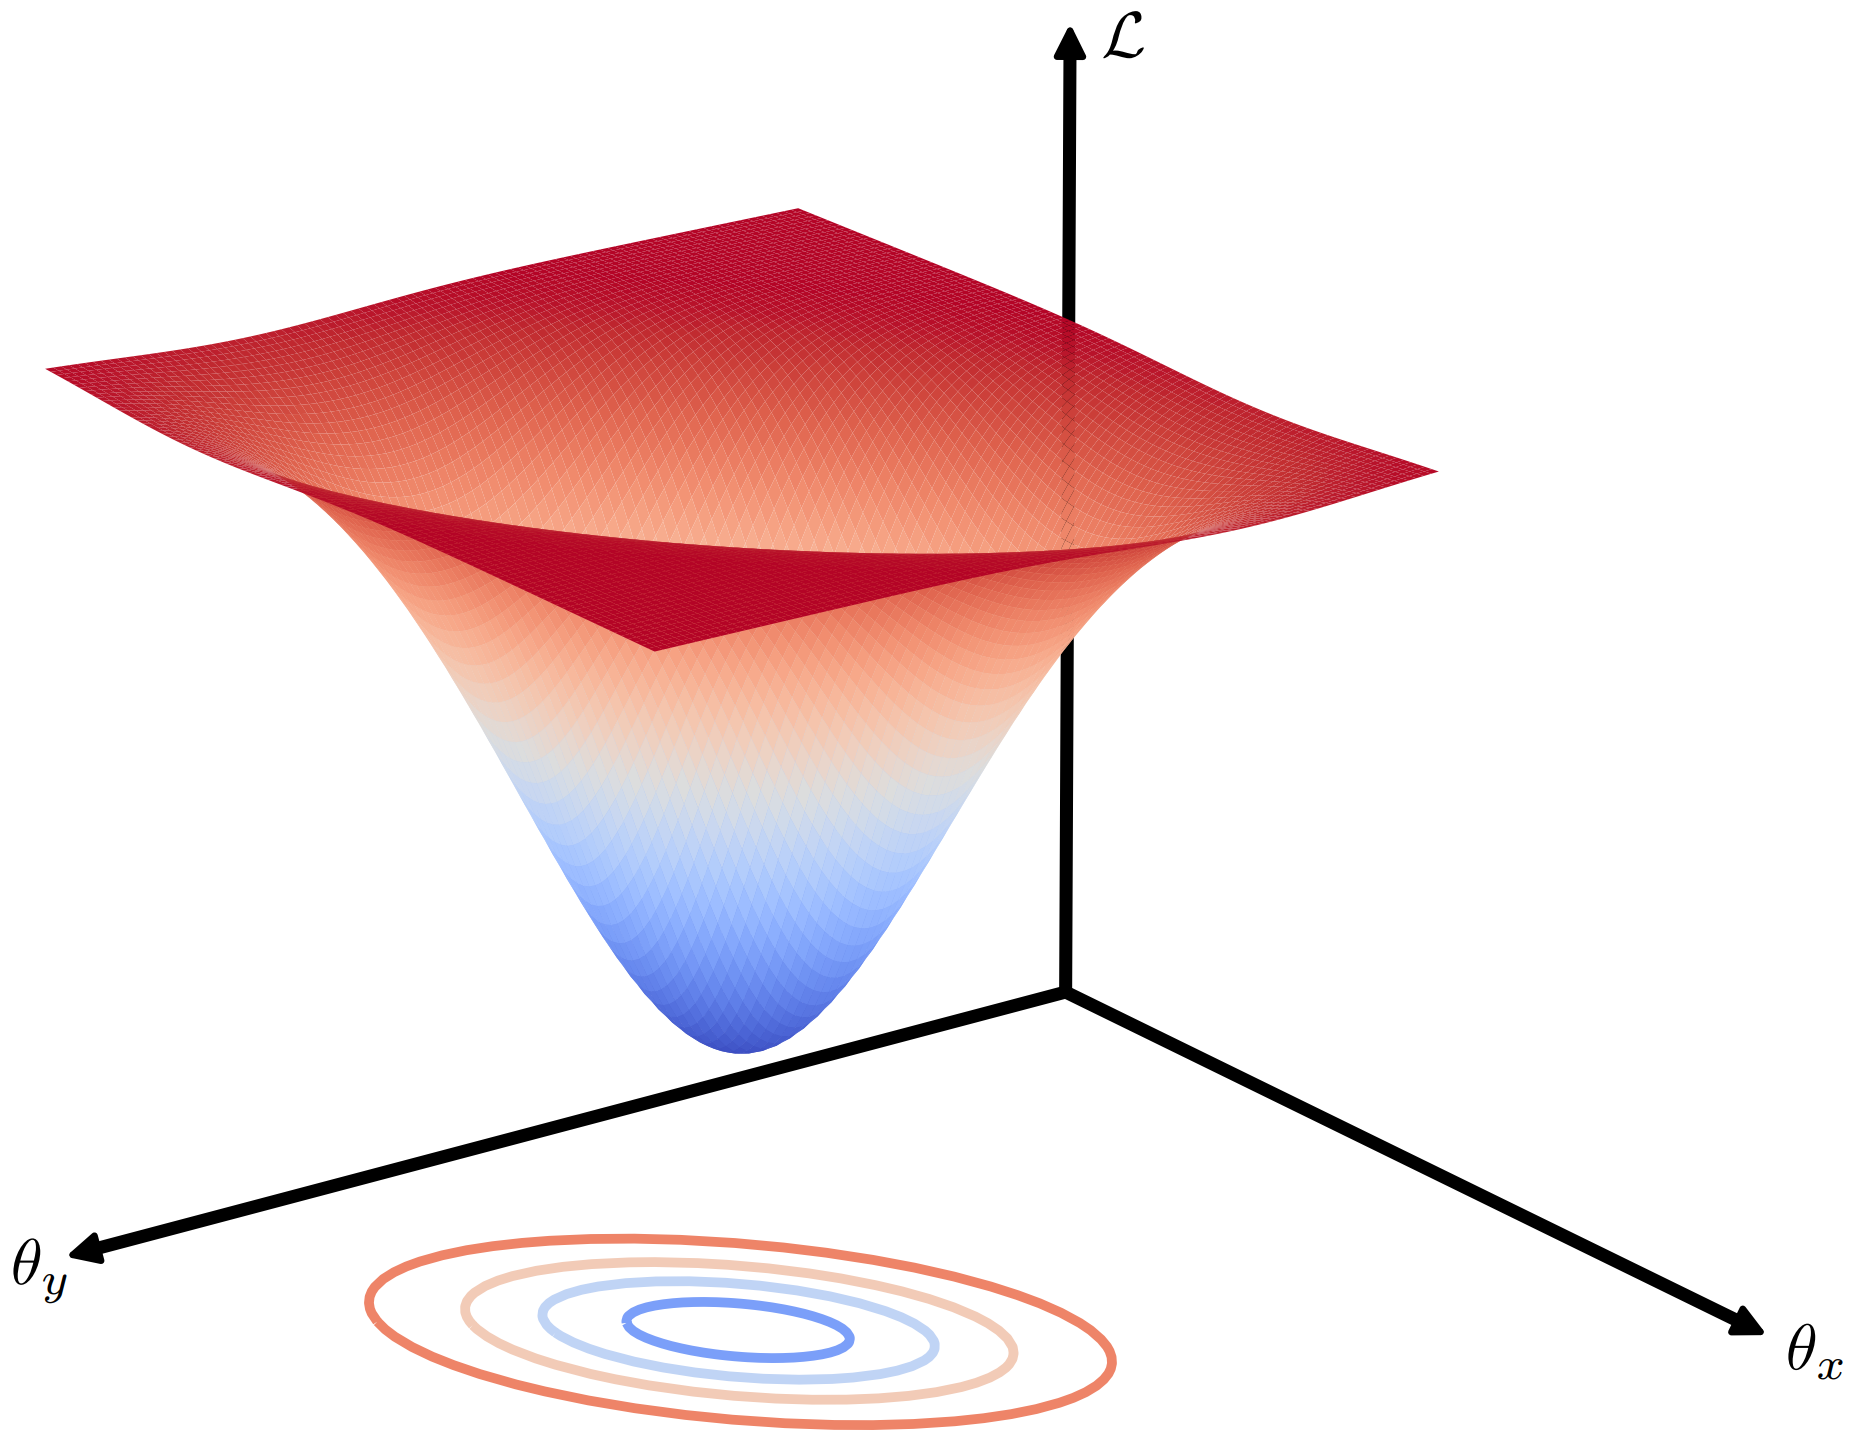
\includegraphics[width=.7\textwidth]{figs/surface.png}
\end{figure}
\vspace{-0.5em}
\begin{figure}
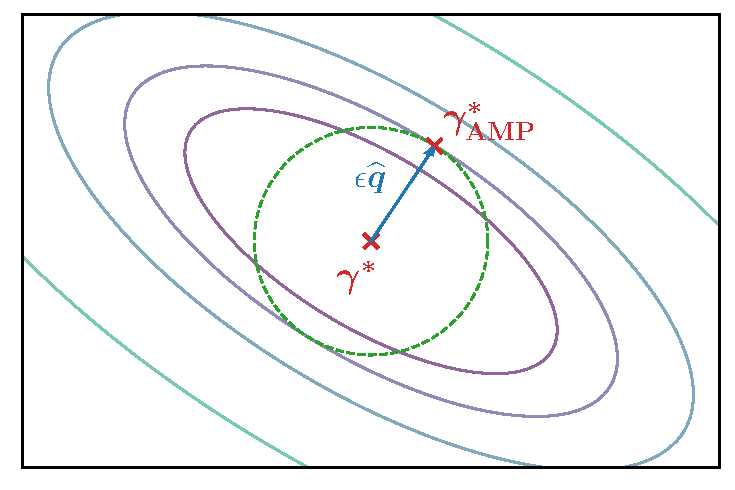
\includegraphics[width=.7\textwidth]{figs/gaussian.pdf}
\caption{The minimum values of $\gamma$ and $\gamma_\mathrm{AMP}$.}
\end{figure}
\end{columns}
\vspace{1em}
\end{frame}

\begin{frame}{AMP Regularizes Gradient Norm}

\begin{theorem}[stated informally]
Let $N=1$. The AMP training is equivalent to ERM training with an additional term:
\begin{equation*}
\widetilde{\mathcal{J}}_\mathrm{ERM}(\boldsymbol{\theta}):=\mathcal{J}_\mathrm{ERM}(\boldsymbol{\theta})+\Omega(\boldsymbol{\theta})
\end{equation*}
where
\begin{equation*}
\Omega(\boldsymbol{\theta}):=\begin{cases}
\zeta\Vert\nabla_{\boldsymbol{\theta}}\mathcal{J}_\mathrm{ERM}(\boldsymbol{\theta})\Vert_2^2,&\Vert\zeta\nabla_{\boldsymbol{\theta}}\mathcal{J}_\mathrm{ERM}(\boldsymbol{\theta})\Vert_2\le\epsilon\\
\epsilon\Vert\nabla_{\boldsymbol{\theta}}\mathcal{J}_\mathrm{ERM}(\boldsymbol{\theta})\Vert_2,&\Vert\zeta\nabla_{\boldsymbol{\theta}}\mathcal{J}_\mathrm{ERM}(\boldsymbol{\theta})\Vert_2>\epsilon
\end{cases}
\end{equation*}
\end{theorem}

% Thus, the AMP training algorithm effectively tries to find the local minima of empirical risk that not only have low values, but also have small gradient norm near the minima. Note that a minimum with smaller gradient norms around it is a flatter minimum.

\end{frame}
